\documentclass[12pt]{book}
\usepackage[utf8]{inputenc}
\usepackage[spanish]{babel}
\usepackage{chronosys}



\title{Calladium}
\author{Libertad Pantoja}
\date{July 2021}

\begin{document}

%%%%%%%%%%%%%%%%%%%%% Cubierta %%%%%%%%%%%%%
\clearpage
%% temporary titles
% command to provide stretchy vertical space in proportion
\newcommand\nbvspace[1][3]{\vspace*{\stretch{#1}}}
% allow some slack to avoid under/overfull boxes
\newcommand\nbstretchyspace{\spaceskip0.5em plus 0.25em minus 0.25em}
% To improve spacing on titlepages
\newcommand{\nbtitlestretch}{\spaceskip0.6em}
\pagestyle{empty}
\begin{center}
\bfseries
\nbvspace[1]
\Huge
{\nbtitlestretch\huge
Calladium}

\nbvspace[1]
\normalsize

Sueños Pandémicos\\
\nbvspace[1]
\small Por\\
\Large Libertad Pantoja\\[0.5em]


\nbvspace[2]

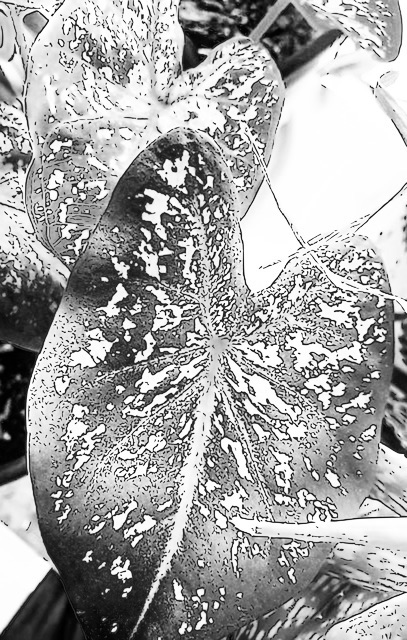
\includegraphics[width=1.5in]{cal.jpeg}
\nbvspace[3]
\normalsize

DOHA\\
\large
PUBLISHED IN THE WILD
\nbvspace[1]
\end{center}
%%%%%%%%%%%%%%%%%%%%%%%%%%%%%%%%%%%%%%%%%%%%%%%%%%%%%%%%%%%%%

\tableofcontents


\chapter{Prólogo}
Lorem ipsum...

\chapter{Línea del tiempo}

\startchronology
\startchronology
[startyear=2019,stopyear=2021]
\chronoevent{2019}{First documented case}
\chronoevent{2021}{Pandemics in Mexico}
\stopchronology


\chapter{Pre-pandemia}

\subsection*{\hfill 15 de abril 2019}

Tengo un jardín amplio en el techo del edificio lleno de helechos y plantas que debo cuidar.

\subsection*{\hfill 20 de abril 2019}

Voy a visitar a mi tío, el rey de Inglaterra, con mi familia y con mi amigo Humberto. El rey y su familia cercana tienen un perro grande que al nacer fue bautizado. El perro está por morir. Le han puesto sus condecoraciones en casa de mis abuelos para mostrárnoslas.
\\
El rey es grande, gordo, barbón. Trae puestos varios collares, uno de ellos de cuentas largas y rojas como chiles. A pesar de que el rey es blanco su hijo mayor, mi primo, es de piel negra. Él es mi compañero y tiene una novia igual a él.

\subsection*{\hfill 21 de abril 2019}

Vivo en un departamento pequeño con mis padres y mi hermana. Hay poco espacio. Esta mañana solo estamos mi mamá, mi hermana y yo. No nos hemos peinado y seguimos en piyama. 
\\
Por la ventana vemos a la vecina del departamento de al lado sentada en su cama, cargando a su bebé. Entra mucha luz por ahí. Decidimos cerrar la ventana para poder dormir.
\\
-Maravilloso, voy a salir despeinada en televisión- dice mi mamá. Ella sabe que estaban grabando en casa de la vecina.


\chapter{Pandemia}

\section{Inicio}

\subsection*{\hfill 22 de abril 2020}

Estoy en un museo con Esther y con sus amigos. El museo es una combinación entre Papalote museo del niño y el Museo de historia natural de la Ciudad de México. Les pido que se adelanten al concierto. Me quedo observando al dinosaurio. El museo está casi vacío. Me detengo a ver hacia un patio interno similar al del Universum.\\
Vamos por un camino sinuoso de tierra en un cañón. El cielo y la tierra son rojizos. Está atardeciendo.

\subsection*{\hfill 28 de junio 2020}
Voy a visitar a Atenea a Durango junto con unas amigas. Durango está a la orilla del mar. 
Atenea es bióloga y nos pide que, antes de ir al evento, 
la ayudemos a sacar los cadáveres que quedaron después del accidente del barco chino. 
Caminamos por las calles de Durango. 
\\
Durango tiene un cielo muy azul, muchos ríos y plantas. Las tiendas chinas son muy populares. 
Nos detenemos un rato a comprar plumas de gel y a pasar al baño.  
Hemos caminado mucho y seguiremos caminando hasta el mar.
\\
Pasamos por un río lleno de insectos de colores,
 bordeado de zacate amarillo y plantas acuáticas. 
 Atenea nos dice que lo malo es que casi todos los insectos 
 que se pueden ver son machos porque las hembras son muy pequeñas. 
 \\
Cuando llegamos a la playa, se está haciendo de noche. Hay redes tendidas en la arena. La luz viene de los barcos, los hoteles y el atardecer. Una de mis amigas y Atenea se ponen a sacar los cadáveres mientras yo cuido las lanchas donde los pondremos. Me quedo dormida. Despierto cuando acaban de terminar de sacar el primer listado de cadáveres. Entonces, llega un señor a preguntar si podemos sacar el segundo listado de cadáveres también. Atenea dice que de ninguna manera y nos vamos. \\
En la playa la gente está pescando. Tienen una charola larga llena de pescados donde se ven algunas tortugas bebés pequeñísimas, moradas con amarillo.


\subsection*{\hfill 16 de noviembre de 2020}
Yo soy caníbal, toda mi familia es caníbal. Me oculto en un supermercado para poder alimentarme y sobrevivir. Ya asesinaron a toda mi familia, sólo quedo yo. Me van a descubrir. Alguien, un señor grande y regordete, me ve. Él se da cuenta de lo que yo soy: una especie de vampiro que no envejece y mata. Él y los humanos que quedan deciden acabar conmigo. Le pido que sea rápido. 
Me llevan a un parque fuera del centro comercial y me ponen de rodillas. Me van a matar de un golpe.  

\subsection*{\hfill 21 de noviembre de 2020}
Rafa abre y cierra una cortina. Entre más la cierra, más trabajo me cuesta respirar. Cada vez que la abre entra una luz anaranjada en la habitación.
27 de diciembre 2020
Quiero dominar los puertos para pescar camarones especiales para hacer un platillo delicioso.
\\
\\
Estoy en C.U. Salgo hacia Copilco para ir a una cafebrería que me gusta mucho. Quiero comprar libros, pero ya tienen muy pocos y no me interesan los que hay. Saludo a un chico que está sentado comiendo. Me da la impresión de que es Mario González Suárez, pero al verlo bien me doy cuenta de mi error y me da mucha pena. Él me saluda con extrañeza, pero con una sonrisa. Yo le pido que me disculpe, le digo que lo confundí con alguien más. Él es barbón y joven.
Salgo de ahí. Voy a buscar otra librería que ya ha salido en mis sueños, pero está cerrada. Hay una mujer en un suéter gris de lana. Es la dueña de una de las librerías.
 
\subsection*{\hfill 24 de julio 2021}
Yo tomo las clases en Literaria con mi tío Mau. Moni, su hermana, trabaja para literaria y nos consigue las sesiones antes. \\
En el trabajo tengo que convertir muchos sitios web en sitios rusos y me siento abrumada porque tal vez tenga que estudiar matemáticas avanzadas.\\
Mau es un niñito. Hay un murciélago.


\end{document}
